%%% lorem.tex --- 
%% 
%% Filename: lorem.tex
%% Description: 
%% Author: Ola Leifler
%% Maintainer: 
%% Created: Wed Nov 10 09:59:23 2010 (CET)
%% Version: $Id$
%% Version: 
%% Last-Updated: Wed Nov 10 09:59:47 2010 (CET)
%%           By: Ola Leifler
%%     Update #: 2
%% URL: 
%% Keywords: 
%% Compatibility: 
%% 
%%%%%%%%%%%%%%%%%%%%%%%%%%%%%%%%%%%%%%%%%%%%%%%%%%%%%%%%%%%%%%%%%%%%%%
%% 
%%% Commentary: 
%% 
%% 
%% 
%%%%%%%%%%%%%%%%%%%%%%%%%%%%%%%%%%%%%%%%%%%%%%%%%%%%%%%%%%%%%%%%%%%%%%
%% 
%%% Change log:
%% 
%% 
%% RCS $Log$
%%%%%%%%%%%%%%%%%%%%%%%%%%%%%%%%%%%%%%%%%%%%%%%%%%%%%%%%%%%%%%%%%%%%%%
%% 
%%% Code:

\chapter{Results}
\label{cha:5-results}
Results from the experiments and parameter values are presented in this chapter. Figures \ref{fig:example_bastar}-\ref{fig:example_randombastar} shows paths in the environment from simulations of the implemented CPP algorithms.

\begin{figure}
    \centering
    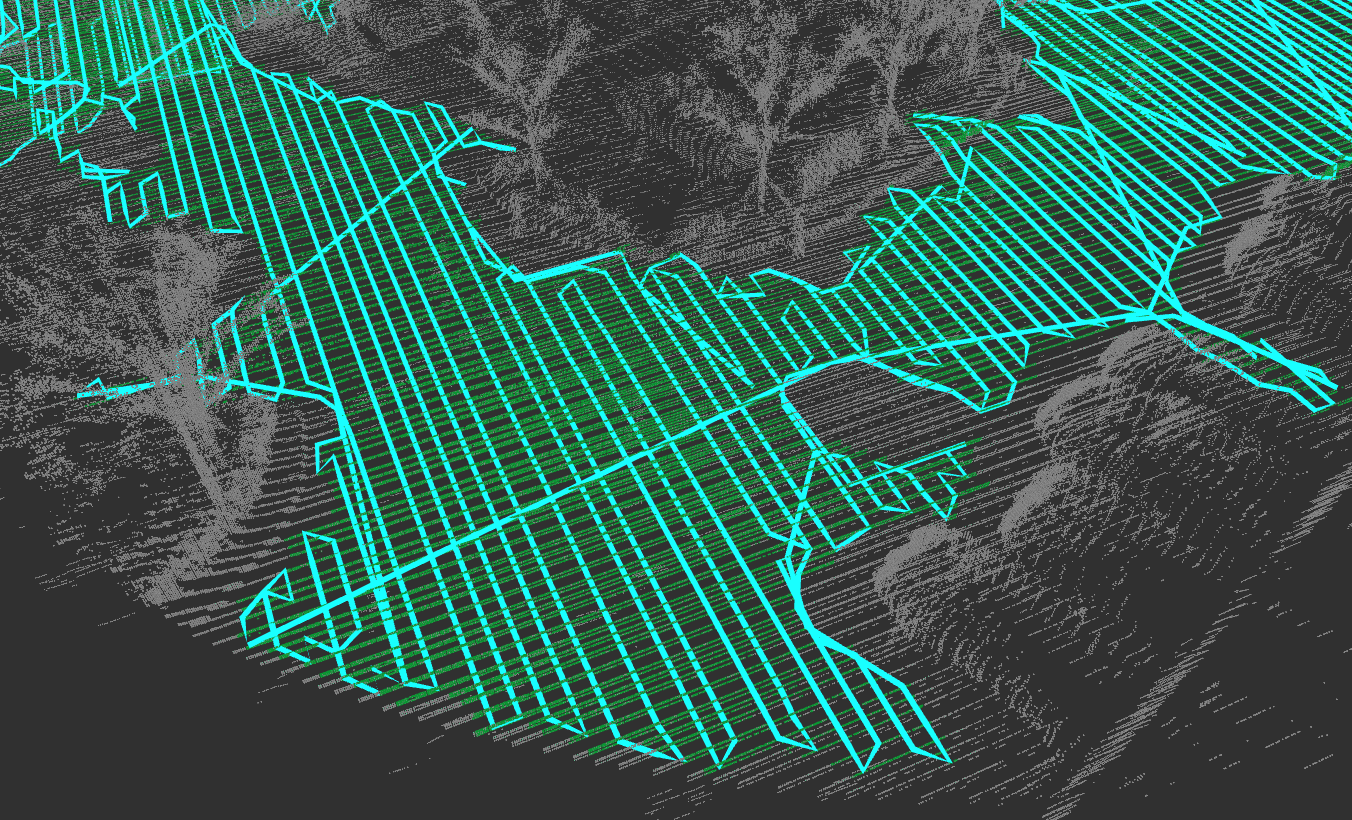
\includegraphics[width=\textwidth]{figures/example_bastar2.png}
    \caption{BA* path from simulations}
    \label{fig:example_bastar}
\end{figure}

\begin{figure}
    \centering
    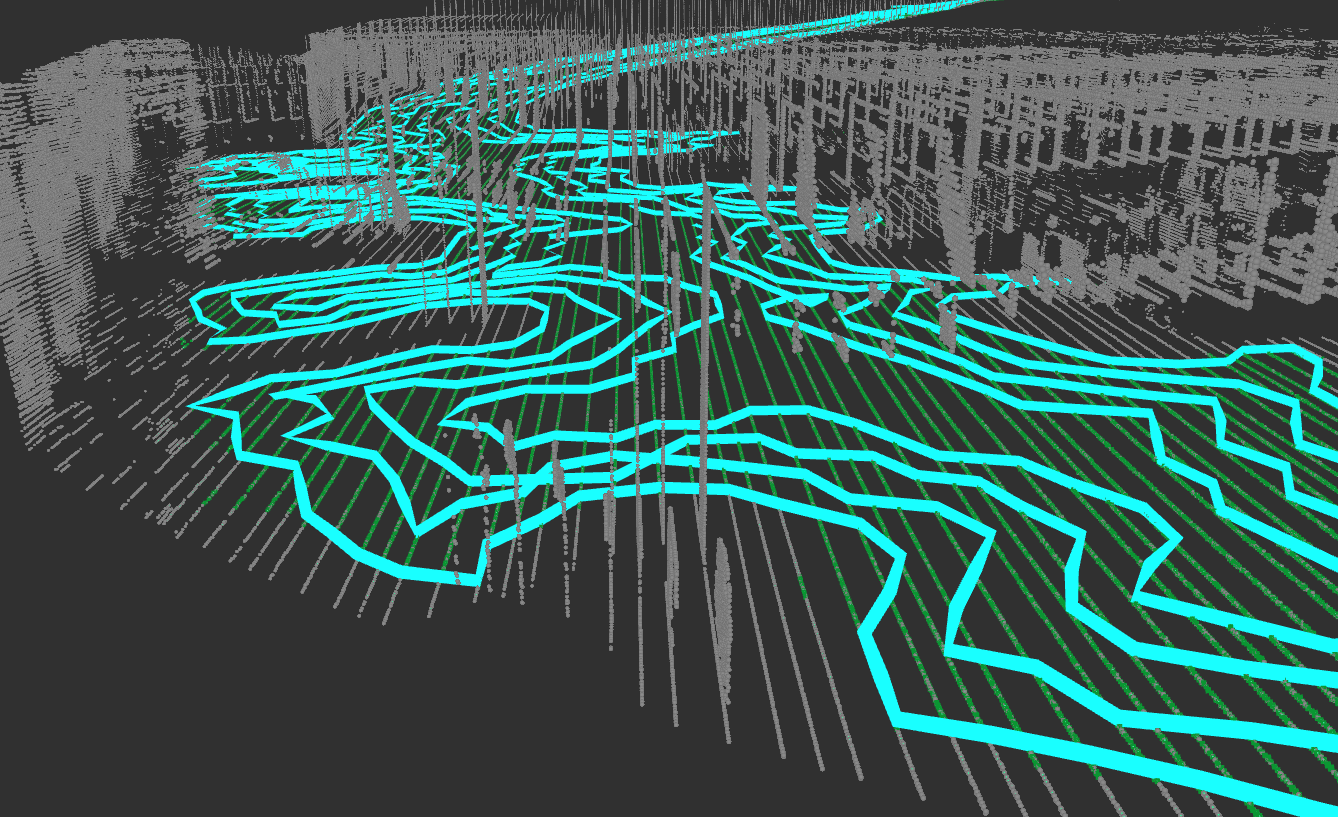
\includegraphics[width=\textwidth]{figures/example_spiral.png}
    \caption{Spiral path from simulations}
    \label{fig:example_spiral}
\end{figure}

\begin{figure}
    \centering
    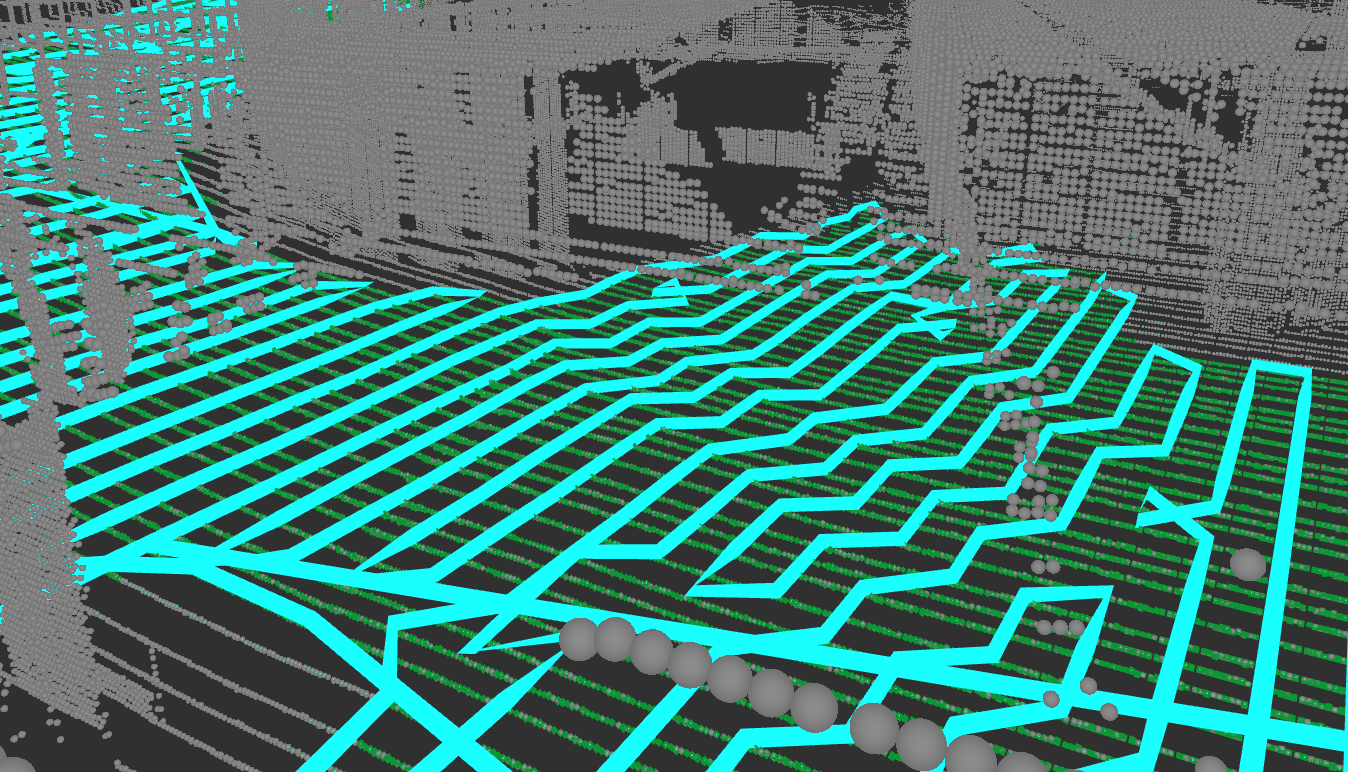
\includegraphics[width=\textwidth]{figures/example_curvedbastar.png}
    \caption{Curved BA* path from simulations}
    \label{fig:example_curvedbastar}
\end{figure}

\begin{figure}
    \centering
    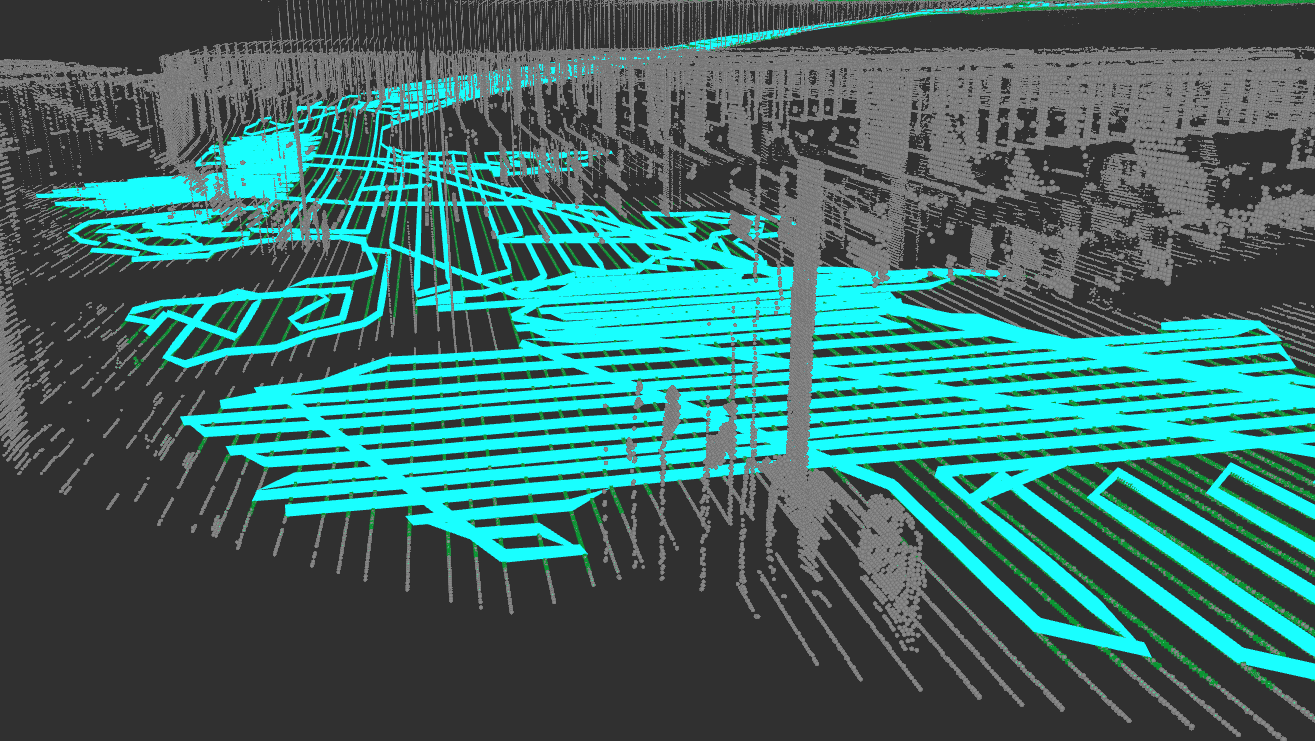
\includegraphics[width=\textwidth]{figures/example_randombastar.png}
    \caption{Sampled BA* \& Inward Spiral path from simulations}
    \label{fig:example_randombastar}
\end{figure}

\section{Parameters}

\subsection{Robot parameters}
Parameters related to the robot are presented in Table \ref{tab:robot_parameters}.

\begin{table}[h!]
    \centering
    \caption{Robot parameters. Values of \emph{Real data} parameters are based on data from the real world provided by the developers of the robot. Values of \emph{Resolution} parameters are minimised to give a good resolution while keeping the computational time on a reasonable level.}
    \begin{tabular}{|c|c|c|c|}
        \hline 
        \textbf{Parameter} & \textbf{Value} & \textbf{Explanation} & \textbf{Based on} \\
        \hline 
        $r_R$ & 0.375 m & Coverage radius & Real data \\
        $\lambda^R_{cov}$ & 0.375 m & Coverage step size & Resolution \\
        \hline 
    \end{tabular}
    
    \label{tab:robot_parameters}
\end{table}

\subsection{Motion Planner parameters}
Parameters for the Motion Planner are presented in Table \ref{tab:mp_parameters}.

\begin{table}[h!]
    \centering
    \caption{Motion Planner parameter. Values of \emph{Resolution} parameters are set to give a good resolution while keeping the computational time on a reasonable level. \emph{Hand tuned based on tests} parameters are hand tuned by making multiple tests and adjust the values to give plausible reliance, computational time and paths.}
    \begin{tabular}{|c|c|c|c|}
        \hline 
        \textbf{Parameter} & \textbf{Value} & \textbf{Explanation} & \textbf{Based on} \\
        \hline 
        $\lambda$ & 0.1 m & Step size & Resolution \\
        $\lambda_{A*}$ & 0.5 m & Step size used in A* & Hand tuned b.o. tests \\
        $\lambda_{RRT}$ & 0.3 m & Step size used in RRT & Hand tuned b.o. tests \\
        $r_{trav}$ & 0.2 m & Threshold for untraversability & Hand tuned b.o. tests \\
        $N^{RRT}_{max}$ & 10 000 & Max iterations in RRT & Resolution \\
        \hline 
    \end{tabular}
    
    \label{tab:mp_parameters}
\end{table}

\subsection{CPP Algorithms parameters}
Parameters for the CPP algorithms are presented in Table \ref{tab:cpp_parameters}.

\begin{table}[h!]
    \centering
    \caption{CPP Algorithms parameters. These values are calculated using the equations in Section \ref{sec:param_calc}.}
    \begin{tabular}{|c|c|c|c|}
        \hline 
        \textbf{Parameter} & \textbf{Value} & \textbf{Explanation} & \textbf{Based on} \\
        \hline 
        $\lambda_{CPP}$ & 0.61 m & Step size in CPP algoithms & Equation \ref{eq:lambda_cpp}\\
        $r_{visited}$ & 0.43 m & Threshold for a position to be visited & Equation \ref{eq:r_visited}\\
        \hline 
    \end{tabular}
    
    \label{tab:cpp_parameters}
\end{table}

\subsection{Sampled BA* \& Inward Spiral parameters}
Parameters for the Sampled BA* \& Inward Spiral used in Experiment 2 are presented in Table \ref{tab:sampled_parameters}.

\begin{table}[h!]
    \centering
    \caption{CPP Algorithms parameters. These values are hand tuned by making multiple tests and adjusting the values to give good results regarding computational time, total rotation, length of path and coverage.}
    \begin{tabular}{|c|c|c|c|}
        \hline 
        \textbf{Parameter} & \textbf{Value} & \textbf{Explanation} & \textbf{Based on} \\
        \hline 
        $r_{sampled}$ & 0.2 m & Threshold for a sampled position to have been visited & Hand tuned b.o. tests \\
        $N^{iter}_{max}$ & 200 & Max iterations of Sampled BA* paths & Hand tuned b.o. tests\\
        $N_{\phi}$ & 4 & Number of angles & Hand tuned b.o. tests\\
        $C_{1}$ & 88\% & Coverage goal for Sampled BA* & Hand tuned b.o. tests\\
        $C_{2}$ & 98\% & Total coverage goal & Hand tuned b.o. tests\\
        $C_{min}$ & 0.5\% & Min. coverage for a BA* segment & Hand tuned b.o. tests\\
        $N_{min}$ & 2 & Min. number of points in a Inward Spiral segment & Hand tuned b.o. tests\\
        
        \hline 
    \end{tabular}
    
    \label{tab:sampled_parameters}
\end{table}

\section{Experiment 1 - BA*, Inward Spiral and Curved BA* over Time}
Results of Experiment 1 is presented in the Figures \ref{fig:exp1_coverage}-\ref{fig:exp1_rotation}. 

\begin{figure}
\centering
    \begin{subfigure}{0.85\textwidth}
    \centering
    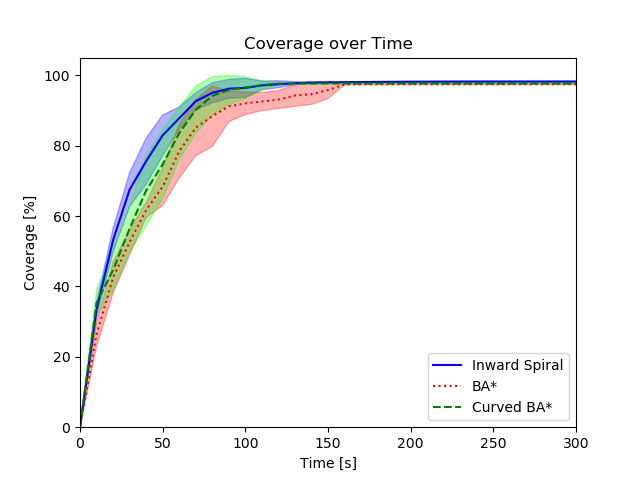
\includegraphics[width=\textwidth]{figures/exp1_coverage.png}
    \caption{Full view.}
    \label{fig:exp1_coverage_full}
    \end{subfigure}
    \begin{subfigure}{0.85\textwidth}
    \centering
    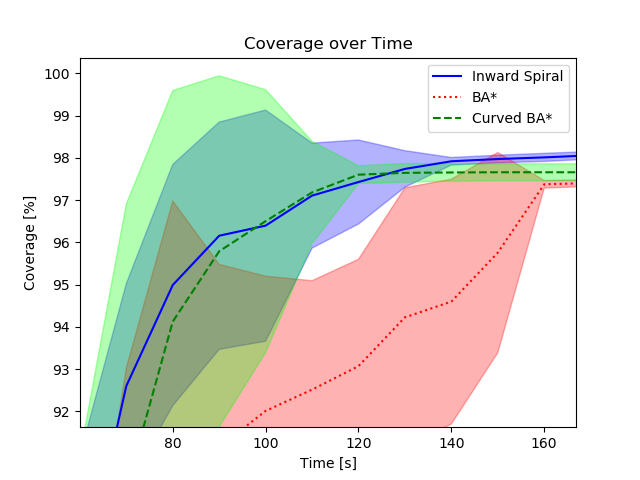
\includegraphics[width=\textwidth]{figures/exp1_coverage_zoom.png}
    \caption{Zoomed in view.}
    \label{fig:exp1_coverage_zoom}
    \end{subfigure}
    \caption{Results of Experiment 1. Means and standard deviations of coverage over time.}
    \label{fig:exp1_coverage}
\end{figure}

\begin{figure}
\centering
    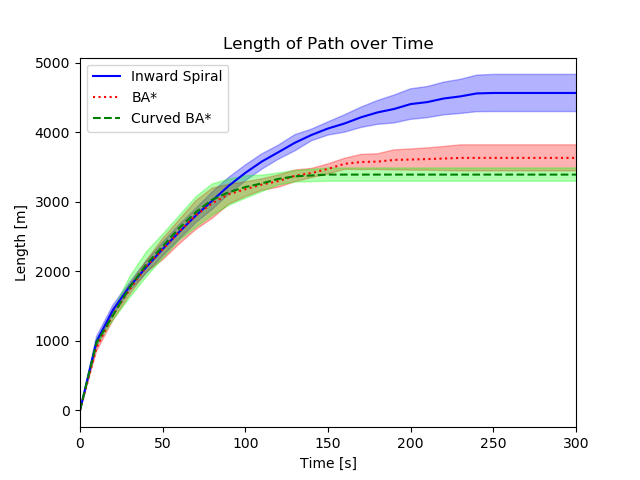
\includegraphics[width=0.85\textwidth]{figures/exp1_length.png}
    \caption{Results of Experiment 1. Means and standard deviations of path length over time.}
    \label{fig:exp1_length}
\end{figure}


\begin{figure}
\centering
    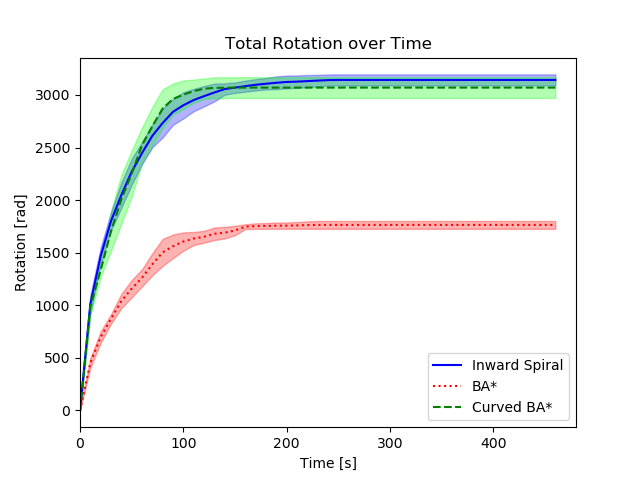
\includegraphics[width=0.85\textwidth]{figures/exp1_rotation.png}
    \caption{Results of Experiment 1. Means and standard deviations of rotation over time.}
    \label{fig:exp1_rotation}
\end{figure}

\section{Experiment 2 - Tuning of $d_{max}$ for Sampled BA* \& Inward Spiral}
Results of Experiment 2 is presented in the Figures \ref{fig:exp2_time}-\ref{fig:exp2_rotation}. The average coverage for all paths in Experiment 2 was 98.3\%. To be able to compare with the algorithms in Experiment 1, their means and standard deviations for computational time, path length and total rotation at 98.3\% from Experiment 1 are shown in the figures as well.

\begin{figure}
\centering
    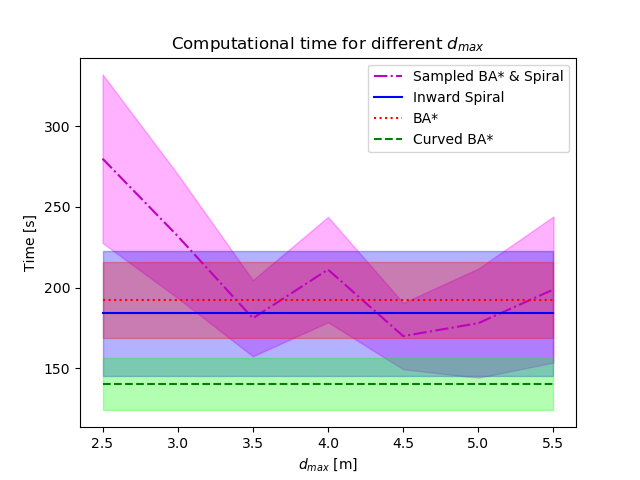
\includegraphics[width=0.85\textwidth]{figures/exp2_time.png}
    \caption{Results of Experiment 2. Means and standard deviations of computational time for different values of parameter $d_{max}$ for Sampled BA* \& Inward Spiral. Means and standard deviations for computational time in Experiment 1 at 98.3\% are shown in the figure as well.}
    \label{fig:exp2_time}
\end{figure}

\begin{figure}
\centering
    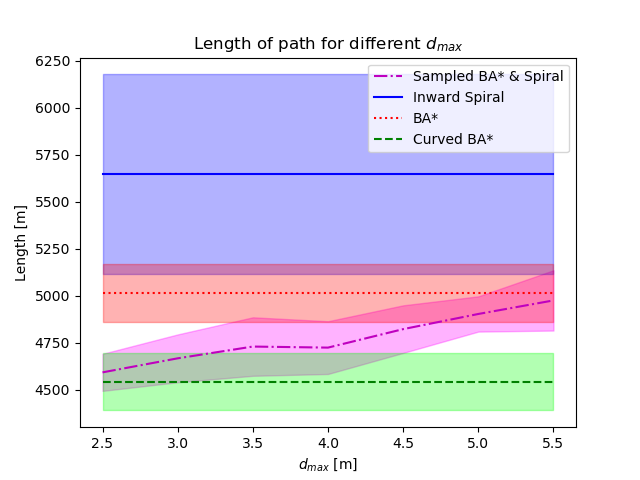
\includegraphics[width=0.85\textwidth]{figures/exp2_length.png}
    \caption{Results of Experiment 2. Means and standard deviations of path length for different values of parameter $d_{max}$ for Sampled BA* \& Inward Spiral. Means and standard deviations for path length in Experiment 1 at 98.3\% are shown in the figure as well.}
    \label{fig:exp2_length}
\end{figure}


\begin{figure}
\centering
    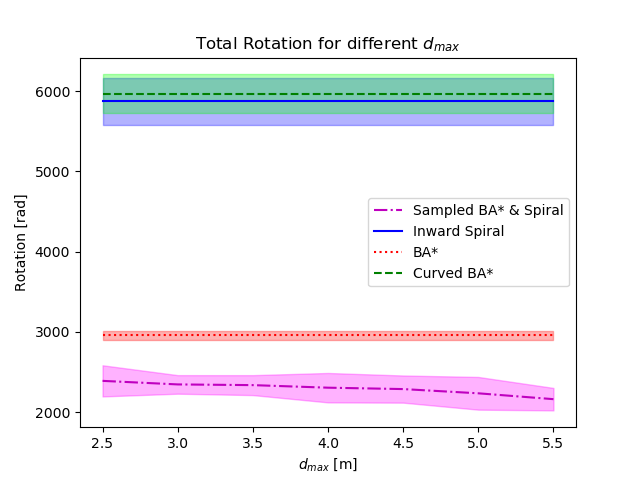
\includegraphics[width=0.85\textwidth]{figures/exp2_rotation.png}
    \caption{Results of Experiment 2. Means and standard deviations of total rotation for different values of parameter $d_{max}$ for Sampled BA* \& Inward Spiral. Means and standard deviations for total rotation in Experiment 1 at 98.3\% are shown in the figure as well.}
    \label{fig:exp2_rotation}
\end{figure}


% \section{Experiment 1 - Maximum coverage}

% Results of the first experiment are presented in figure \ref{fig:max_coverage}. The lowest reached percentage among BA*, BA* Variant and Inward Spiral were 97.6\%. RRT for coverage ath planning did not reach a satisfying coverage percentage and were consequently excluded in Experiment 2.

% \begin{figure}
%     \centering
%     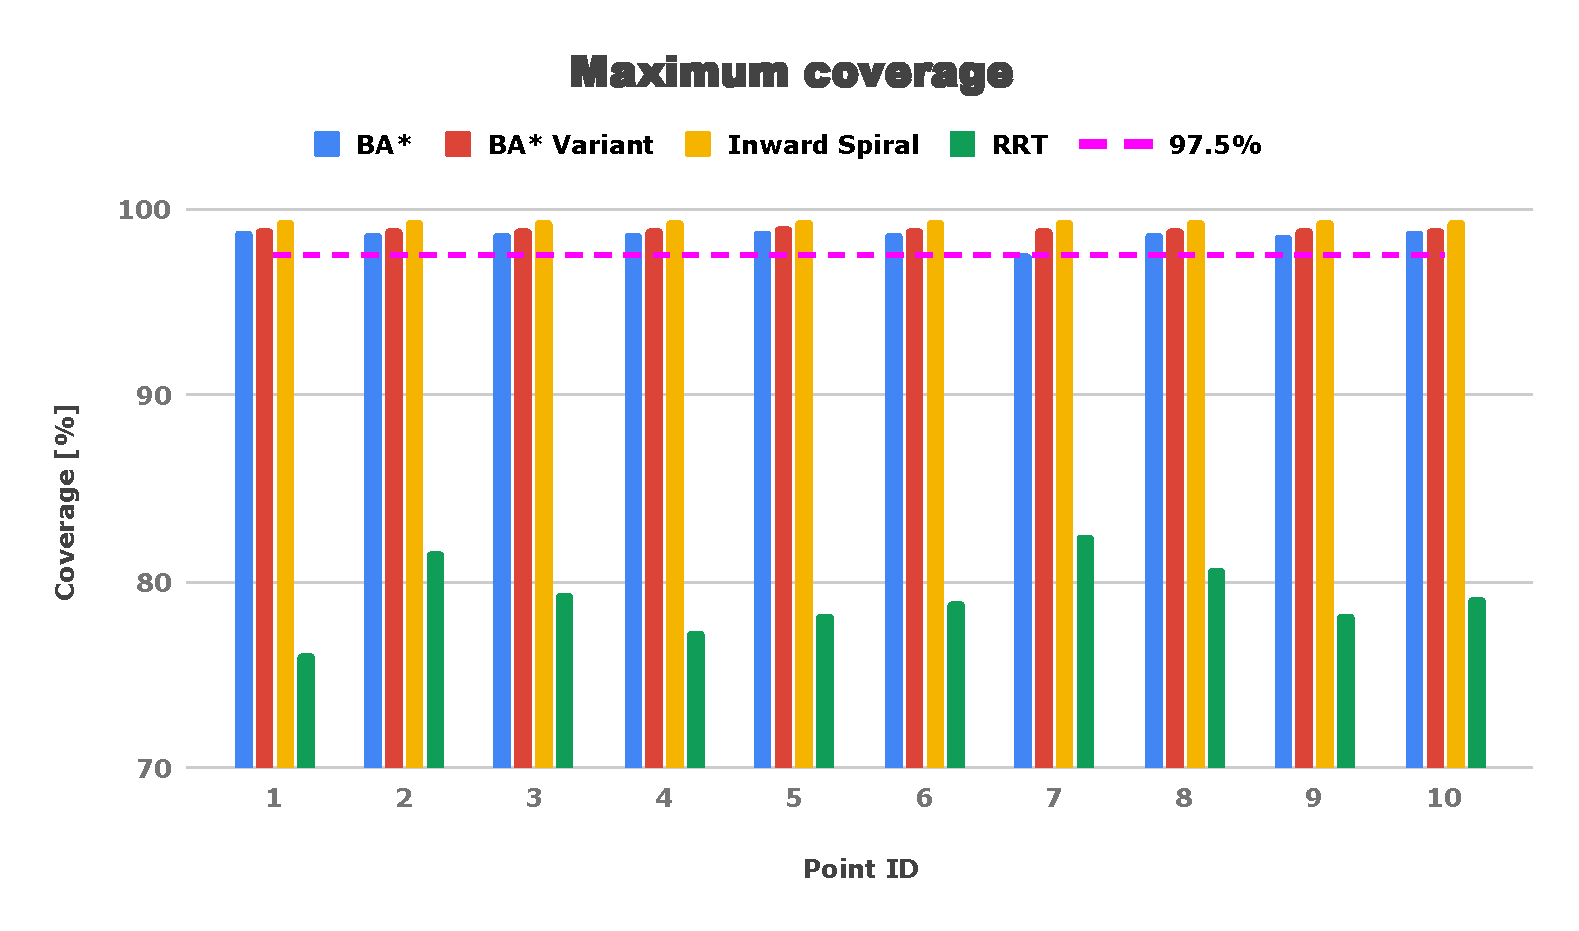
\includegraphics[width=0.99\textwidth]{figures/Maximum coverage .pdf}
%     \caption{Results of Experiment 1. The maximum possible coverage for the four CPP algorithms with a limit of 6 minutes.}
%     \label{fig:max_coverage}
% \end{figure}

% \section{Experiment 2 - Efficiency and Effectiveness}

% Based on the results in experiment 1 the goal coverage was set to 97.5\%. The BA*, BA* Variant and Inward Spiral algorithms planned covering paths until the goal coverage was reached. The length of the path, total rotation and computational time were calculated according to \ref{sec:properties} are presented in figures \ref{fig:length_of_path}-\ref{fig:computational_time}. The horizontal lines in the figures represent the average value for each algorithm.

% \begin{figure}
%     \centering
%     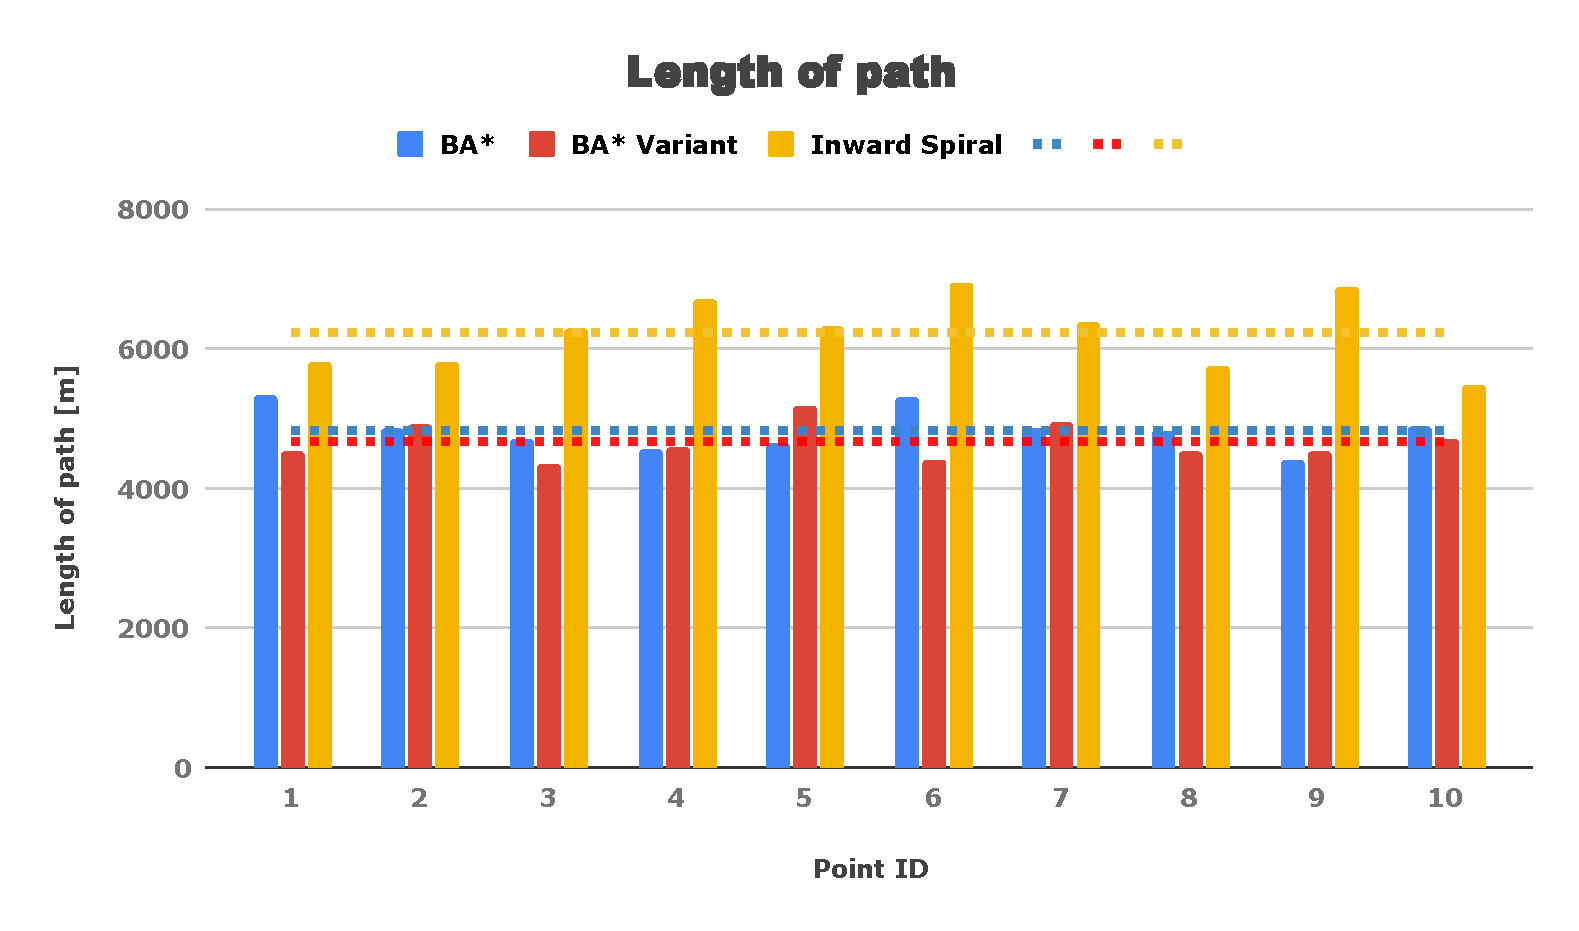
\includegraphics[width=0.99\textwidth]{figures/Length of path.pdf}
%     \caption{Results of Experiment 2. The length of the generated paths. The horizontal dotted lines represent the average value of the corresponding algorithm.}
%     \label{fig:llength_of_path}
% \end{figure}


% \begin{figure}
%     \centering
%     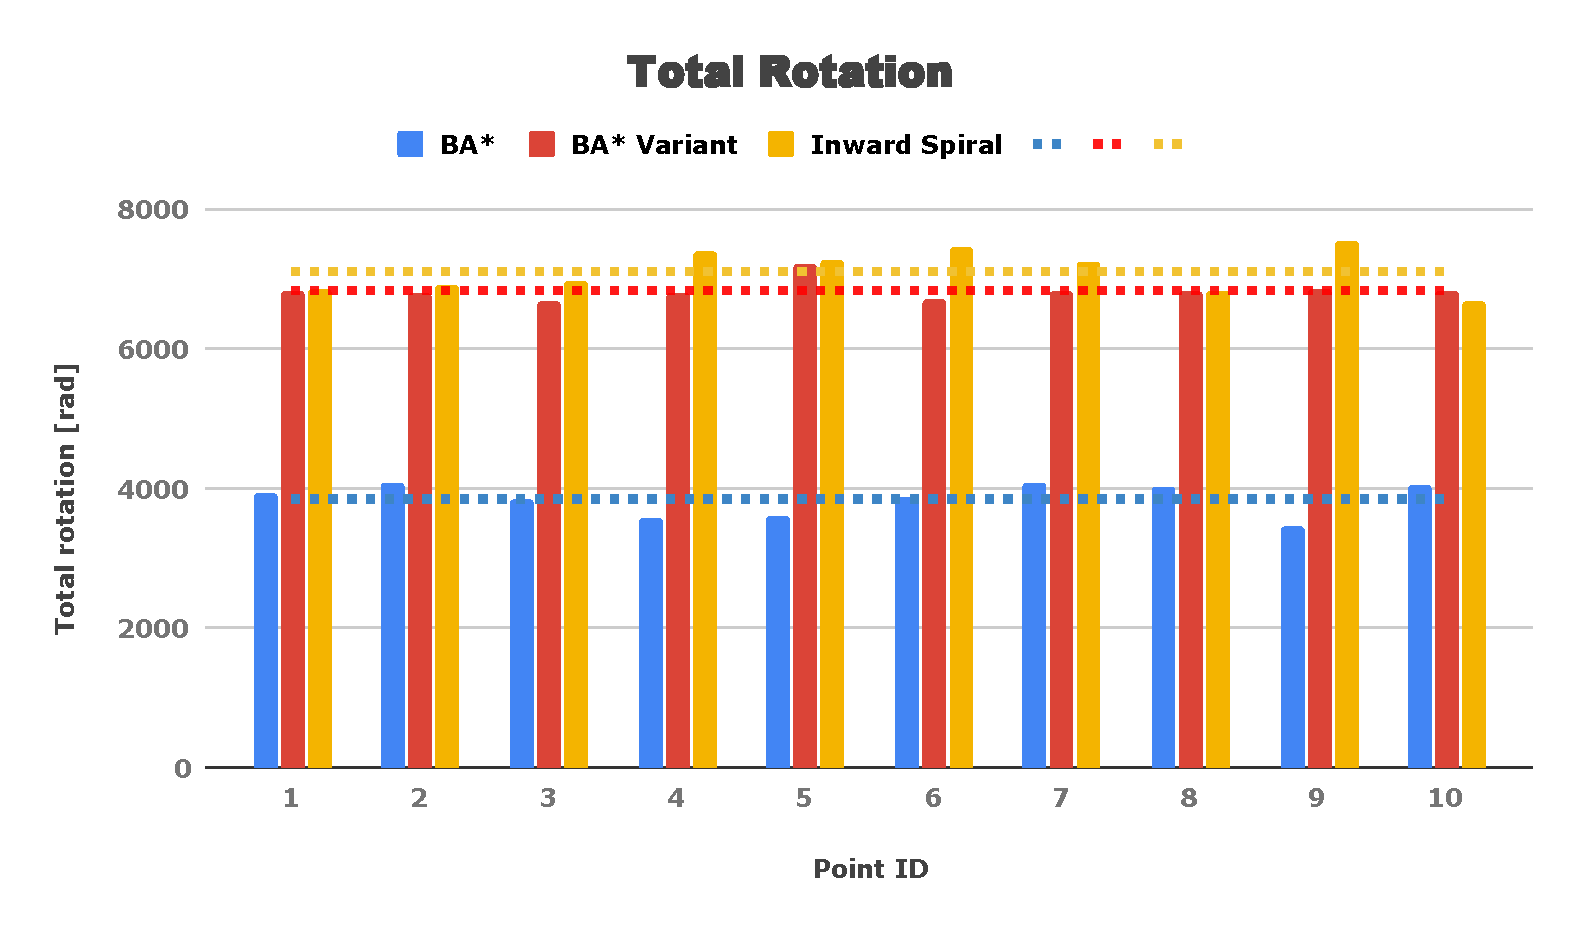
\includegraphics[width=0.99\textwidth]{figures/Total Rotation.pdf}
%     \caption{Results of Experiment 2. The total rotation of the paths. The horizontal dotted lines represent the average value of the corresponding algorithm.}
%     \label{fig:total_rotation}
% \end{figure}

% \begin{figure}
%     \centering
%     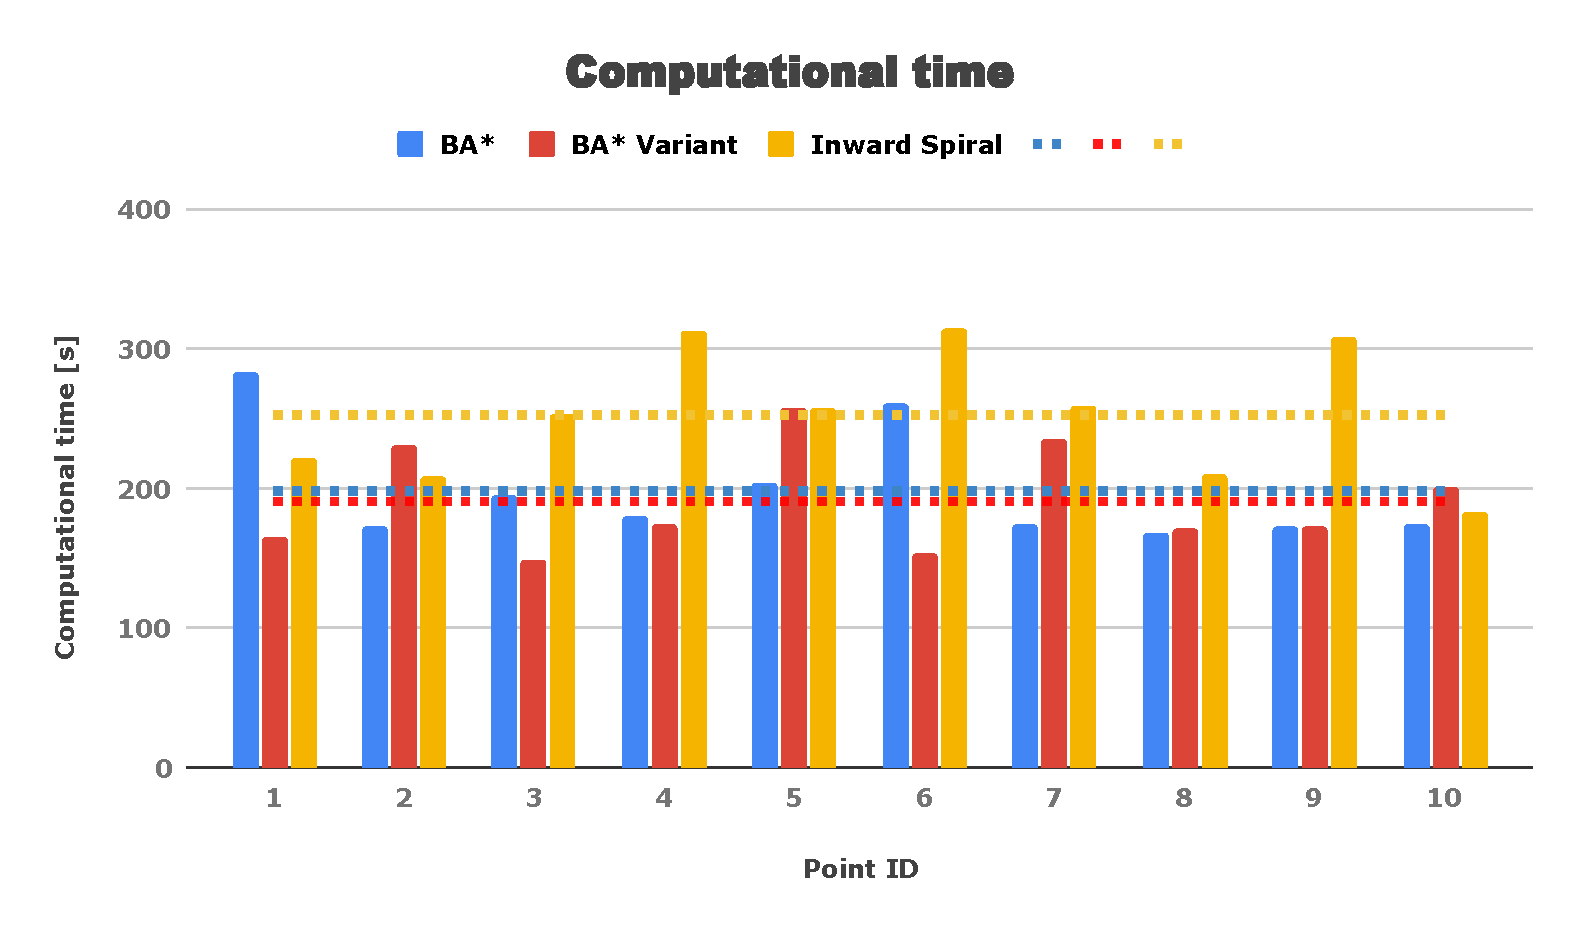
\includegraphics[width=0.99\textwidth]{figures/Computational time.pdf}
%     \caption{Results of Experiment 2. Computational time to generate a path that reaches the goal coverage for each algorithm. The horizontal dotted lines represent the average value of the corresponding algorithm.}
%     \label{fig:computational_time}
% \end{figure}

% \section{Experiment 3 - Sampled BA* \& Spiral}

% The same coverage goal was used in experiment 3 as in experiment 2. The parameters of the Sampled BA* \& Spiral algorithm were hand tuned to keep the computational time close to the times in experiment 2, see figure \ref{fig:exp3_computational_time} while minimizing the length of the path and the total rotation. 

% In figures \ref{fig:exp3_length_of_path} and \ref{fig:exp3_total_rotation} the Sampled BA* and Spiral is compared with the results of BA* and BA* variant in experiment 2.

% \begin{figure}
%     \centering
%     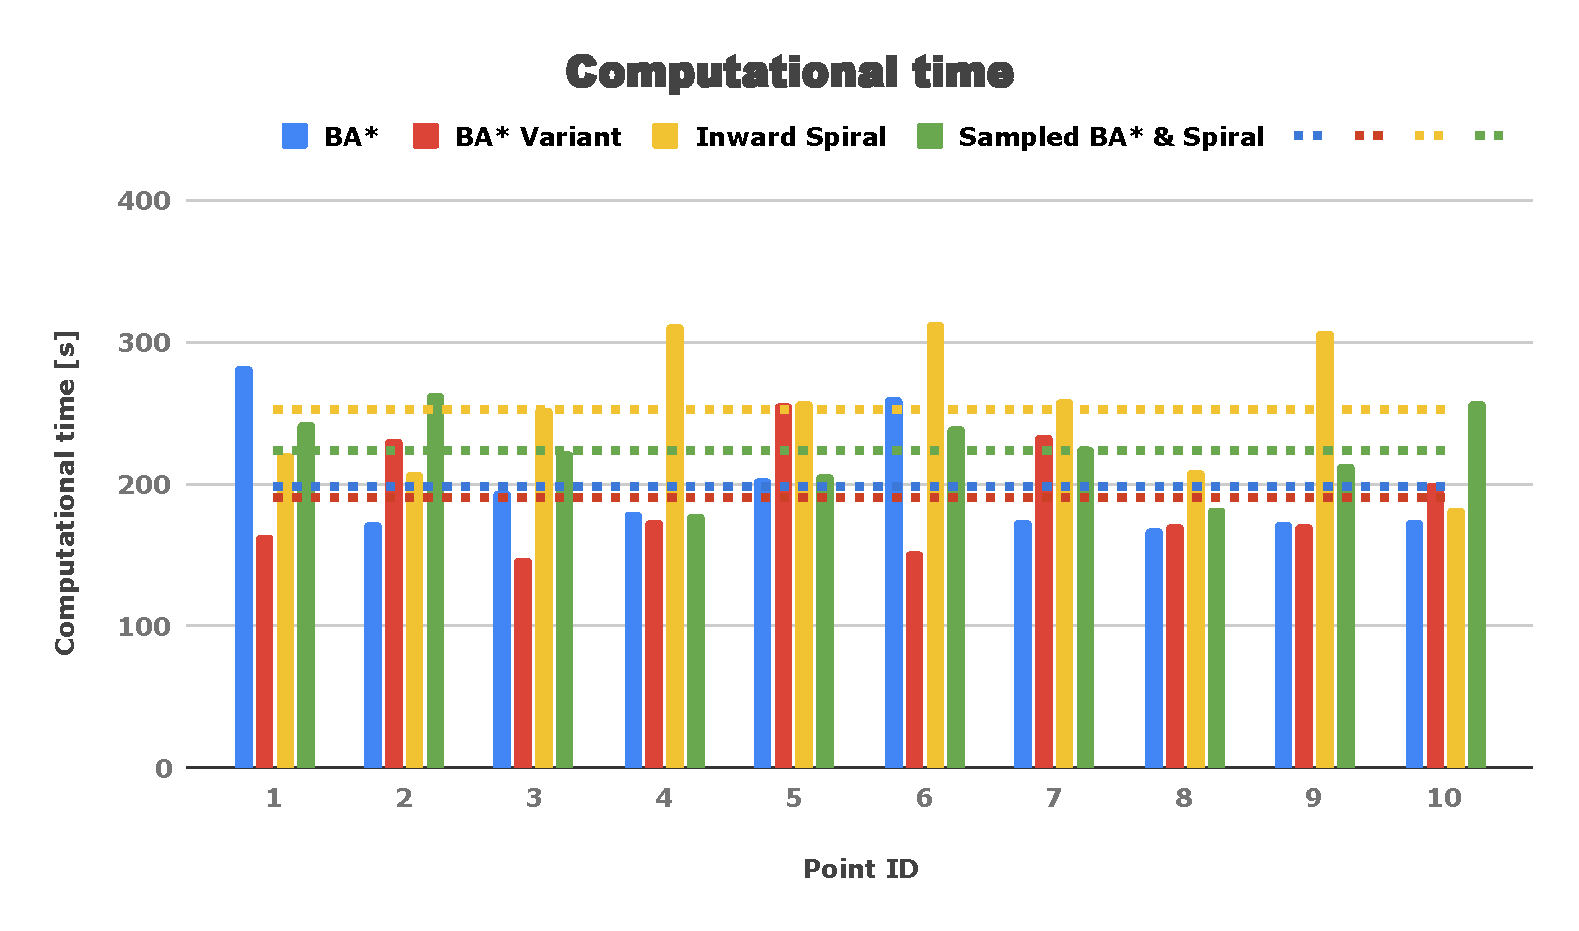
\includegraphics[width=0.99\textwidth]{figures/Computational time(1).pdf}
%     \caption{Results of Experiment 3. Shows that  computational times of the Sampled BA* & Spiral is close to the computational times of the other algorithms in experiment 2. The horizontal dotted lines represent the average value of the corresponding algorithm.}
%     \label{fig:exp3_computational_time}
% \end{figure}


% \begin{figure}
%     \centering
%     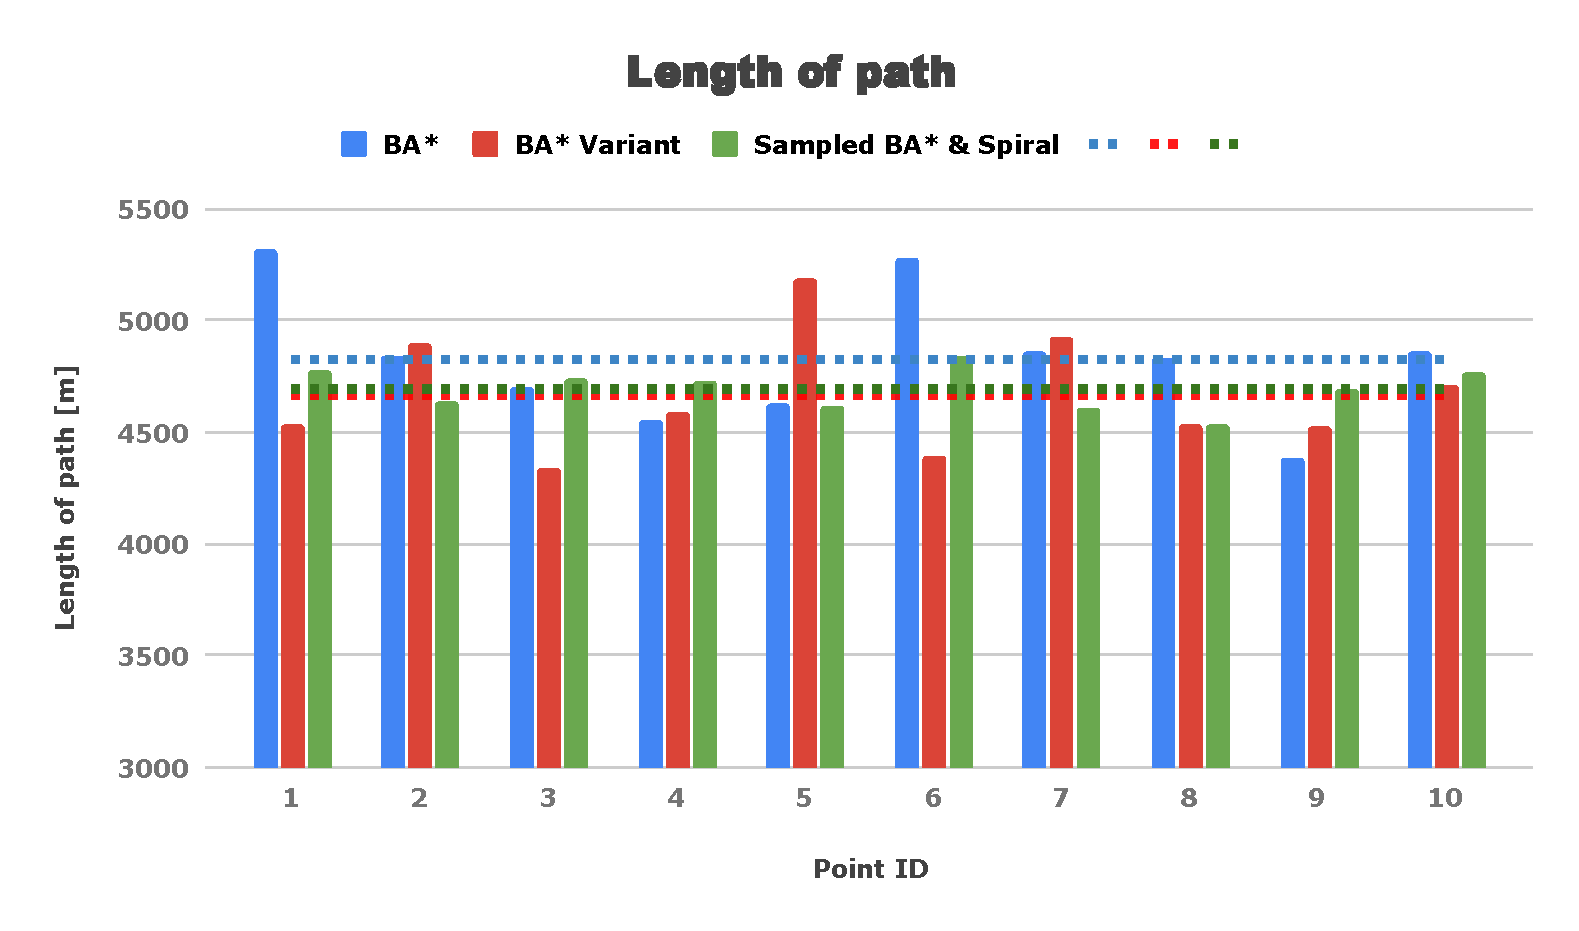
\includegraphics[width=0.99\textwidth]{figures/Length of path(1).pdf}
%     \caption{Results of Experiment 3. The length of the generated paths. The horizontal dotted lines represent the average value of the corresponding algorithm.}
%     \label{fig:exp3_length_of_path}
% \end{figure}


% \begin{figure}
%     \centering
%     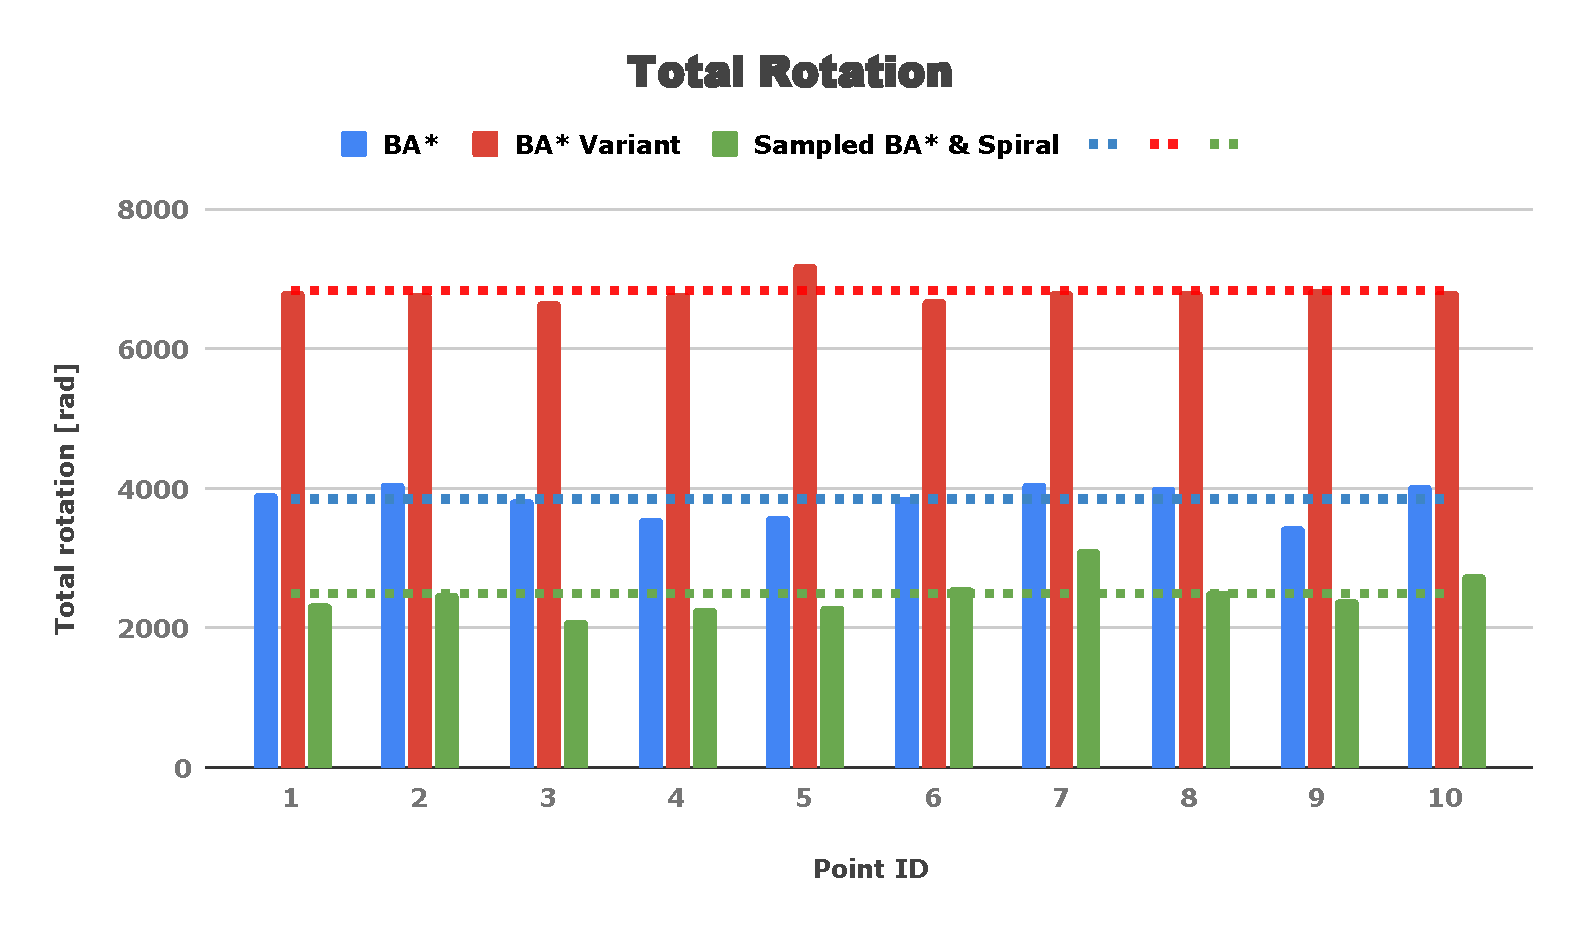
\includegraphics[width=0.99\textwidth]{figures/Total Rotation(1).pdf}
%     \caption{Results of Experiment 3. The total rotation of the paths. The horizontal dotted lines represent the average value of the corresponding algorithm.}
%     \label{fig:exp3_total_rotation}
% \end{figure}





% This chapter presents the results. Note that the results are presented
% factually, striving for objectivity as far as possible.  The results
% shall not be analyzed, discussed or evaluated.  This is left for the
% discussion chapter.

% In case the method chapter has been divided into subheadings such as
% pre-study, implementation and evaluation, the result chapter should
% have the same sub-headings. This gives a clear structure and makes the
% chapter easier to write.

% In case results are presented from a process (e.g. an implementation
% process), the main decisions made during the process must be clearly
% presented and justified. Normally, alternative attempts, etc, have
% already been described in the theory chapter, making it possible to
% refer to it as part of the justification.

%%%%%%%%%%%%%%%%%%%%%%%%%%%%%%%%%%%%%%%%%%%%%%%%%%%%%%%%%%%%%%%%%%%%%%
%%% lorem.tex ends here

%%% Local Variables: 
%%% mode: latex
%%% TeX-master: "demothesis"
%%% End: 
